%%% Time-stamp: <2023-07-20 18:44:27 vladimir>
% %%% Copyright (C) 2019-2023 Vladimir G. Ivanović
% %%% Author: Vladimir G. Ivanović <vladimir@acm.org>
% %%% ORCID: https://orcid.org/0000-0002-7802-7970

\chapter{Findings}\label{ch:findings}\noindent
\bigskip%

This chapter will present the data found using the approach outlined in \prettyref{ch:methods} with the goal of answering my research question: Has Rocketship structured itself and its finances, to earn a return to investors, focusing especially on real estate transactions, and if so, how?

The first section will give a potted history\footnote{''A potted history is brief, a quick summary. Potted meat is meat, usually not of the highest quality, processed and preserved in a tin. The expression is often used in a derogatory way\ldots'' — bobro in \url{https://english.stackexchange.com/questions/237443/what-does-potted-history-mean}} of Rocketship in \prettyref{sec:history}, including a section on how Rocketship has structured itself. 

Since real estate is so important for Rocketship, the next section, \prettyref{sec:location-and-property-info} will lay out what facilities Rocketship has, where those facilities are located, when they were acquired, and what real estate rights Rocketship has over those properties.

%%%%%%%%%%%%%%%%%%%%%%%%%%%%%%%%%%%%%%%%%%%%%%%%%%%%%%%%%%%%%%%%%%%%%%%%%%%%%%%
%%% Rocketship History %%%
%%%%%%%%%%%%%%%%%%%%%%%%%%%%%%%%%%%%%%%%%%%%%%%%%%%%%%%%%%%%%%%%%%%%%%%%%%%%%%%
\section{Rocketship History}\label{sec:history}\indent

\subsection{Rocketship's Corporate Structure}\label{sec:rocketship-corp-struct}\indent

Rocketship's corporate structure was designed from the start to separate schools and their operation from facilities and their construction and maintenance. Rocketship Education is the parent company, a 501(3)(c) non-profit. It owns all the schools, themselves non-profits, plus Launchpad Development Company, another non-profit. Launchpad Development's role is to own all the facilities, one non-profit LLC per location. This structure is diagrammed in \prettyref{fig:RSED-corporate-structure}.

\begin{figure}[ht]
  \centering
  \caption{\normalfont\emph{Rocketship's Corporate Structure (Santa Clara County only) Schools}}\label{fig:corporate-structure}
  \sffamily
  \begin{forest}
    for tree={grow'=east, folder, draw, align=left}
    [ \textbf{Rocketship Education}, baseline
      [ Launchpad Development Company
        [ \textit{Launchpad (LP)}, xshift=4em ]
        [ \textit{Launchpad Development One LLC (LLC1)}, xshift=4em ]
        [ \textit{Launchpad Development Two LLC (LLC2)}, xshift=4em ]
        [ \textit{Launchpad Development Threee LLC (LLC3)}, xshift=4em ]
        [ \textit{Launchpad Development Four LLC (LLC4)}, xshift=4em ]]
      [ Rocketship Support Network (RSN) ]
      [ Rocketship Mateo Sheedy Elementary (RSM) ]
      [ Rocketship Sí-Se-Puede Academy (RSSP) ]
      [ Rocketship Mosaic Elementary (ROMO) ]
      [ Rocketship Discovery Prep (RDP) ]
      [ Rocketship Brilliant Minds (RBM) ]
      [ Rocketship Alma Academy (RSA) ]
      [ Rocketship Spark Academy (RSK) ]
      [ Rocketship Rising Stars (RRS) ]]
    \end{forest}
  \end{figure}

\section{Charter School Financing}\label{sec:findings-charter-financing}\indent

\subsection{Charter School Financial Documents}\label{sec:findings-charter-financial-docs}\indent

\subsubsection{Petitions \& Renewals}\label{sec:petitions-renewals}\indent

The current number of pages of initial and renewal petitions runs to 7371 pages for just Rocketship schools in Santa Clara County.\footnote{The massive size of some of these petition calls into question whether authorizers read them in their entirety.}

\subsubsection{Authorizer Staff Reports}\label{sec:findings-authorizer-staff-reports}\indent

\subsubsection{Budgets, Interim Reports, and CAFRs}\label{sec:findings-budgets-etc}\indent

\subsubsection{LCAPs,}\label{sec:findings-lcaps}\indent

\subsubsection{Board and Committee Supporting Material}\label{sec:findings-board-material}\indent

\section{Charter Schools and Real Estate}\label{sec:findings-charter-real-estate}\indent

\subsection{Rocketship Locations and Property Information}\label{sec:location-and-property-info}\indent

\begin{table}[thb]
  \caption[Rocketship Property Information]{\textit{Rocketship Property Information}}\label{tab:locations}\SingleSpacing%
  \begin{tabular}{lll}
    \toprule
    School          & Address                               & Property Information \\
    \midrule
    Mateo Sheedy    & 788 Locust St., San José, CA 95110    & \prettyref{sec:mateo-sheedy-info} \\
    Sí Se Puede     & 2249 Dobern Ave, San José, CA 95116   & \prettyref{sec:sí-se-puede-info} \\
    Los Sueños      & 331 S. 34th St, San José, CA 95116    & \prettyref{sec:los-suenos-info} \\
    Discovery Prep  & 370 Wooster Ave, San José, CA 95116   & \prettyref{sec:discover-prep-info} \\
    Mosaic          & 950 Owsley Ave, San José, CA 95122    & \prettyref{sec:mosaic-info} \\
    Brilliant Minds & 2960 Story Rd, San José, CA 95127     & \prettyref{sec:brilliant-minds-info} \\
    Alma Academy    & 198 West Alma Ave, San José, CA 95110 & \prettyref{sec:alma-academy-info} \\
    Spark Academy   & 683 Sylvandale Ave San José, CA 95111 & \prettyref{sec:spark-academy-info} \\
    Fuerza          & 70 S. Jackson Ave, San José, CA 95116 & \prettyref{sec:fuerza-info} \\
    Rising Stars    & 3173 Senter Road, San José, CA 95111  & \prettyref{sec:rising-stars-info} \\
    \bottomrule
  \end{tabular}
\end{table}

\subsection{Facilities Options}\label{sec:findings-facilities-options}\indent

\subsubsection{Co-Locating}\label{sec:findings-co-locating}\indent

\subsubsection{Leasing}\label{sec:findings-leasing}\indent

\subsubsection{Owning}\label{sec:findings-owning}\indent

\subsection{Funding Facility Ownership}\label{sec:findings-funding-ownership}\indent

\subsubsection{Private Funding, Loans, and Foundation Grants}\label{sec:findings-private-funding}\indent

\subsubsection{Venture Funds}\label{sec:findings-venture-funds}\indent

\subsubsection{Tax Credits}\label{sec:findings-tax-credits}\indent

The New Market Tax credit of 39\% (5\% for the first 3 years, and 6\% for the remaining 4 years) can be applied to taxes due from other investments. Since there is a compounding effect, the 39\% is actually worth over 41\% of the initial investment. Note that these other investment may themselves have a return. With these kinds of incentives, it's no wonder that the New Markets Tax Credit is popular. But one should not be deceived into thinking that just because New Markets Tax Credits must be made in economically depressed area that investors are investing out of the goodness of their heart. The tax credit investment is nearly without risk because the tax credit is guaranteed as long as the charter school remains open. If the school stays open for seven years, the risk is zero.

\subsubsection{Bonds}\label{sec:findings-bonds}\indent

 Three bond prospectuses total over 1000 pages.    

% \subsection{Real Estate Data}\label{sec:real-estate-data}\indent
% \begin{enumerate}
%   \item What is the actual price, date, and buyer \& seller information for each property?
%   \item What is the legal relationship between Rocketship Education and Launchpad Development?
%   \item How were Rocketship facilities in Santa Clara County financed?
%   \item What are the type and terms of all bonds.
%   \begin{enumerate}
%     \item What bonds were floated: type, rate, \& terms; guaranteed by whom or how? If the bonds are not privatedly placed, they are classed as securities, and their prospectuses are filed with the Securities Exchange Commission and are publicly viewable.
%     \item For conduit bonds, the California Department of Education or Department of Finance web sites 
%   \end{enumerate}
%   \item Enumerate all known leases and their terms. Was part of the lease payment paid by California?
%   \item Enumerate all known loans.
%   \begin{enumerate}[a.]
%     \item What was used as collateral? 
%     \item What were the terms?
%   \end{enumerate}    
%   \item Enumerate donations from foundations and individuals.
%   \item Enumerate venture fund investments.
% \end{enumerate}


% Forms which have been filed with a government entity:
%  \begin{enumerate}
%   \item Federal 990 forms to check against financial statements. IRS maintained. Should cross-reference the financial statements.
%   \item Annual and interim budgets submitted to the California Department of Education.
%   \item Petition approvals and renewals submitted to local school districts, the SCCOE, or the California State Board of Education.

%   The Santa Clara County Office of Education (SCCOE), and each school district in which Rocketship petitioned to open a school has some data/notes from one or more board meetings in which the petition or renewal was discussed. These data might have been presented by Rocketship or by county or district staff. Sometimes there is also public comment.
  
% Often, petitions presented to a school district have been denied and appealed to the Santa Clara County Board of Education, and in a few cases, to California's State Board of Education.
  
%   \item There is some published material on Rocketship.
%   \begin{enumerate}[a.]
%     \item Some books have been written about Rocketship
%     \item Roxana has two ScoopIt collections on Rocketship on and charter schools.
%     \item The ``Stop Rocketship'' web site has lots of information on Rocketship.
%     \item Several academics have datasets of school or district financial information  which include Rocketship.
%     \item Numerous articles, web sites, and blog postings include Rocketship financial data.
%   \end{enumerate}
%   \item Other, outside entities that may add revenue to Rocketship
%   \begin{enumerate}
%     \item Zeal
%     \item Dreambox Learning
%   \end{enumerate}
% \end{enumerate}


\section{Other Data}\label{sec:findings-other-data}\indent

\subsection{Datasets}\label{sec:findings-datasets}\indent

\subsection{State and Federal Filings}\label{sec:findings-state-federal-filings}\indent

\subsection{Curated Social Media}\label{sec:findings-curated-social-media}\indent


\section{Gaps and Anomalies}\label{sec:findings-gaps-anomolies}\indent

Since a goal of this dissertation is to map the flow of money into and out of Rocketship, I will use diagrams similar to the one used by \citeauthor{Baker.Miron2015} (\citeyear{Baker.Miron2015}), which is reproduced here as \prettyref{fig:opresflows}.

\subsection{Triangulation}\label{sec:findings-triangulation}\indent

These data represent the monies that are flowing into Rocketship/Launchpad related to facilities, real estate, bonds, loans, and donations and not tied to the number of students. Once that's been assembled, roll up into one spreadsheet, Rocketship's consolidated financial statements for the fourteen years (2008--2022). The consolidated financial statements can then be compared against the known real estate, bond, loan, and donation transactions. Noe where data is missing or where it conflicts with the consolidated financial statements.

\begin{figure}[ht]
  \centering
  \caption[Operating Resource Flows]{\textit{Operating Resource Flows}}\label{fig:opresflows}
  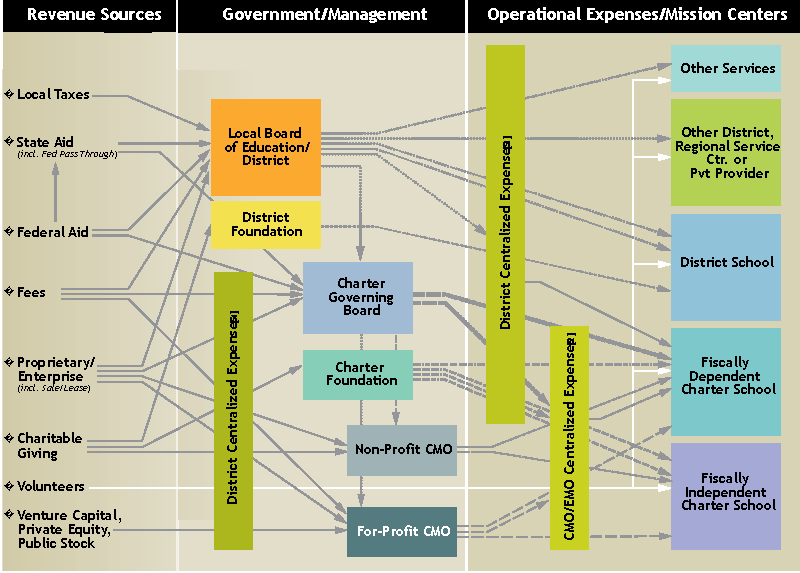
\includegraphics[width=\textwidth]{Operating_Resource_Flows}\\
  \footnotesize\raggedright\textcite[16]{Baker.Miron2015}.
\end{figure}
In this example, money flows from left to right, and there are no loops. Colors are used merely to distinguish the various blocks.


%%% Local Variables:
%%% mode: latex
%%% TeX-master: "Rocketship_Education-An_Exploratory_Public_Policy_Case_Study"
%%% End:
